\documentclass[10 pt,usenames,dvipsnames, oneside]{article}
\usepackage{../../modelo-fracoes}
\graphicspath{{../../../Figuras/licao05/}}


\begin{document}

\begin{center}
  \begin{minipage}[l]{3cm}

\includegraphics[width=2cm]{../../../Figuras/logo}       
\end{minipage}\hfill
\begin{minipage}[r]{.8\textwidth}
 {\Large \scshape Atividade: }  
\end{minipage}
\end{center}
\vspace{.2cm}

\ifdefined\prof
%Caixa do Para o Professor
\begin{goals}
%Objetivos específicos
\begin{enumerate}
    \item       Entender o processo de determinação de um denominador comum entre duas frações com base na ideia de subdivisão da unidade da qual ambas sejam múltiplas inteiras, obtida a partir de um processo geométrico e, a partir desse denominador comum, gerar frações equivalentes às frações dadas e, a partir desse denominador comum, gerar frações equivalentes às frações dadas;
    \item       Determinar a soma de duas frações a partir dessa subdivisão da unidade e da noção de equivalência de frações.
\end{enumerate}

\tcblower

%Orientações e sugestões
\begin{itemize}
    \item       Uma vez estabelecida uma       {\bf unidade}       (no caso, o tamanho da fita), a determinação de uma subdivisão dá origem a um processo de medida por meio de uma       {\bf dupla contagem}, em que estão envolvidas:       {\bf a unidade}, associada ao número~1, com base na qual são contadas quantidades inteiras;       {\bf subdivisões da unidade em partes iguais}       (no caso, os pedaços coloridos das fitas), cuja contagem permite medir quantidades menores que a unidade.
    \item       A atividade envolve a subdivisão de fitas coloridas em pedaços de mesmo tamanho. É recomendável que o professor desenvolva a atividade em sala de aula utilizando materiais concretos. As fitas coloridas podem ser feitas com papel e cartolina, e os alunos podem recortá-las e juntar os pedaços de acordo com o que é pedido nos itens da atividade. Nesta etapa de familiarização inicial com as operações com frações, a manipulação concreta é importante para a construção de significado.
    \item       O item a) visa ao reconhecimento pelo aluno das frações envolvidas na situação apresentada. Assim, espera-se que o aluno responda,       $\frac{1}{3}$,       $\frac{1}{2}$       e~$\frac{1}{4}$.
    \item       Em seguida, é apresentada uma situação simples em que uma subdivisão comum, no caso o pedaço de fita amarelo, permite a determinação da soma:
\end{itemize}
\end{goals}

\bigskip
\begin{center}
{\large \scshape Atividade}
\end{center}
\fi

A professora Estela quer enfeitar sua sala de aula para uma festa da escola. Para isso ela comprou várias fitas, todas de mesmo tamanho, nas cores vermelho, azul e amarelo.

\begin{center}
\begin{tikzpicture}[x=1.0cm,y=1.0cm, scale=.5]
\draw[fill=attention] (0.,1) rectangle (12.,3.);
\draw[fill=common] (0.,-2) rectangle (12.,0.);
\draw[fill=light] (0.,-5) rectangle (12.,-3.);
\end{tikzpicture}
\end{center}


A professora cortou cada fita vermelha em 3 partes iguais, cada fita azul em 2 partes iguais e cada fita amarela em 4 partes iguais.

\begin{center}
\begin{tikzpicture}[x=1.0cm,y=1.0cm, scale=.5]
\draw[fill=attention] (0.,1) rectangle (12.,3.);
\foreach \x in {4,8} \draw[dashed] (\x,1) -- (\x,3);
\draw[fill=common] (0.,-2) rectangle (12.,0.);
\draw[dashed] (6,-2) -- (6,0);
\draw[fill=light] (0.,-5) rectangle (12.,-3.);
\foreach \x in {3,6,9} \draw[dashed] (\x,-5) -- (\x,-3);
\end{tikzpicture}
\end{center}

\begin{enumerate}
  \item     A que fração da fita original corresponde cada pedaço recortado pela professora Estela?
\end{enumerate}

 Em seguida, a professora Estela começou a juntar pedaços recortados das fitas, formando novas fitas coloridas. Ela começou juntando (de forma intercalada) um pedaço azul e dois pedaços amarelos.     \mbox{} \newline

\begin{center}
\begin{tikzpicture}[x=1.0cm,y=1.0cm, scale=.5]
\draw[fill=light] (0.,0) rectangle (3,2);
\draw[fill=common] (3,0) rectangle (9.,2.);
\draw[fill=light] (9,0) rectangle (12,2);
\end{tikzpicture}
\end{center}

Ela verificou que a nova fita formada tinha o mesmo tamanho da fita original. Isso aconteceu porque cada pedaço azul tem o mesmo tamanho de dois pedaços amarelos. Podemos representar o tamanho da nova fita formada pela professora por meio de uma {\bf soma de frações}. Cada pedaço azul corresponde a $\frac{1}{2}$ da fita original. Cada pedaço amarelo corresponde a $\frac{1}{4}$ da fita original, então 2 pedaços amarelos correspondem a $\frac{2}{4}$ da fita original. Portanto, o tamanho da nova fita é igual a: $$\dfrac{1}{2} + \dfrac{2}{4}.$$ Mas, como $\frac{2}{4}$ é igual a $\frac{1}{2}$ (cada pedaço azul tem o mesmo tamanho de dois pedaços amarelos), então: $$\dfrac{1}{2} + \dfrac{2}{4} = \dfrac{1}{2} + \dfrac{1}{2}.$$ O resultado dessa soma $\frac{1}{2} + \frac{1}{2}$ é igual 2 pedaços de $\frac{1}{2}$, isto é, $\frac{2}{2}$ (que é igual 1). Assim: $$\dfrac{1}{2} + \dfrac{2}{4} = \dfrac{1}{2} + \dfrac{1}{2} = 1.$$ Neste caso, o resultado 1 corresponde ao tamanho da fita original.

\begin{enumerate}\setcounter{enumi}{1}
 \item A professora também agrupou pedaços de fita, juntando 1 pedaço amarelo e 1 pedaço azul, como na figura a seguir. A qual fração da fita inicial correspondem esses dois pedaços juntos?
\end{enumerate} %s

\begin{center}
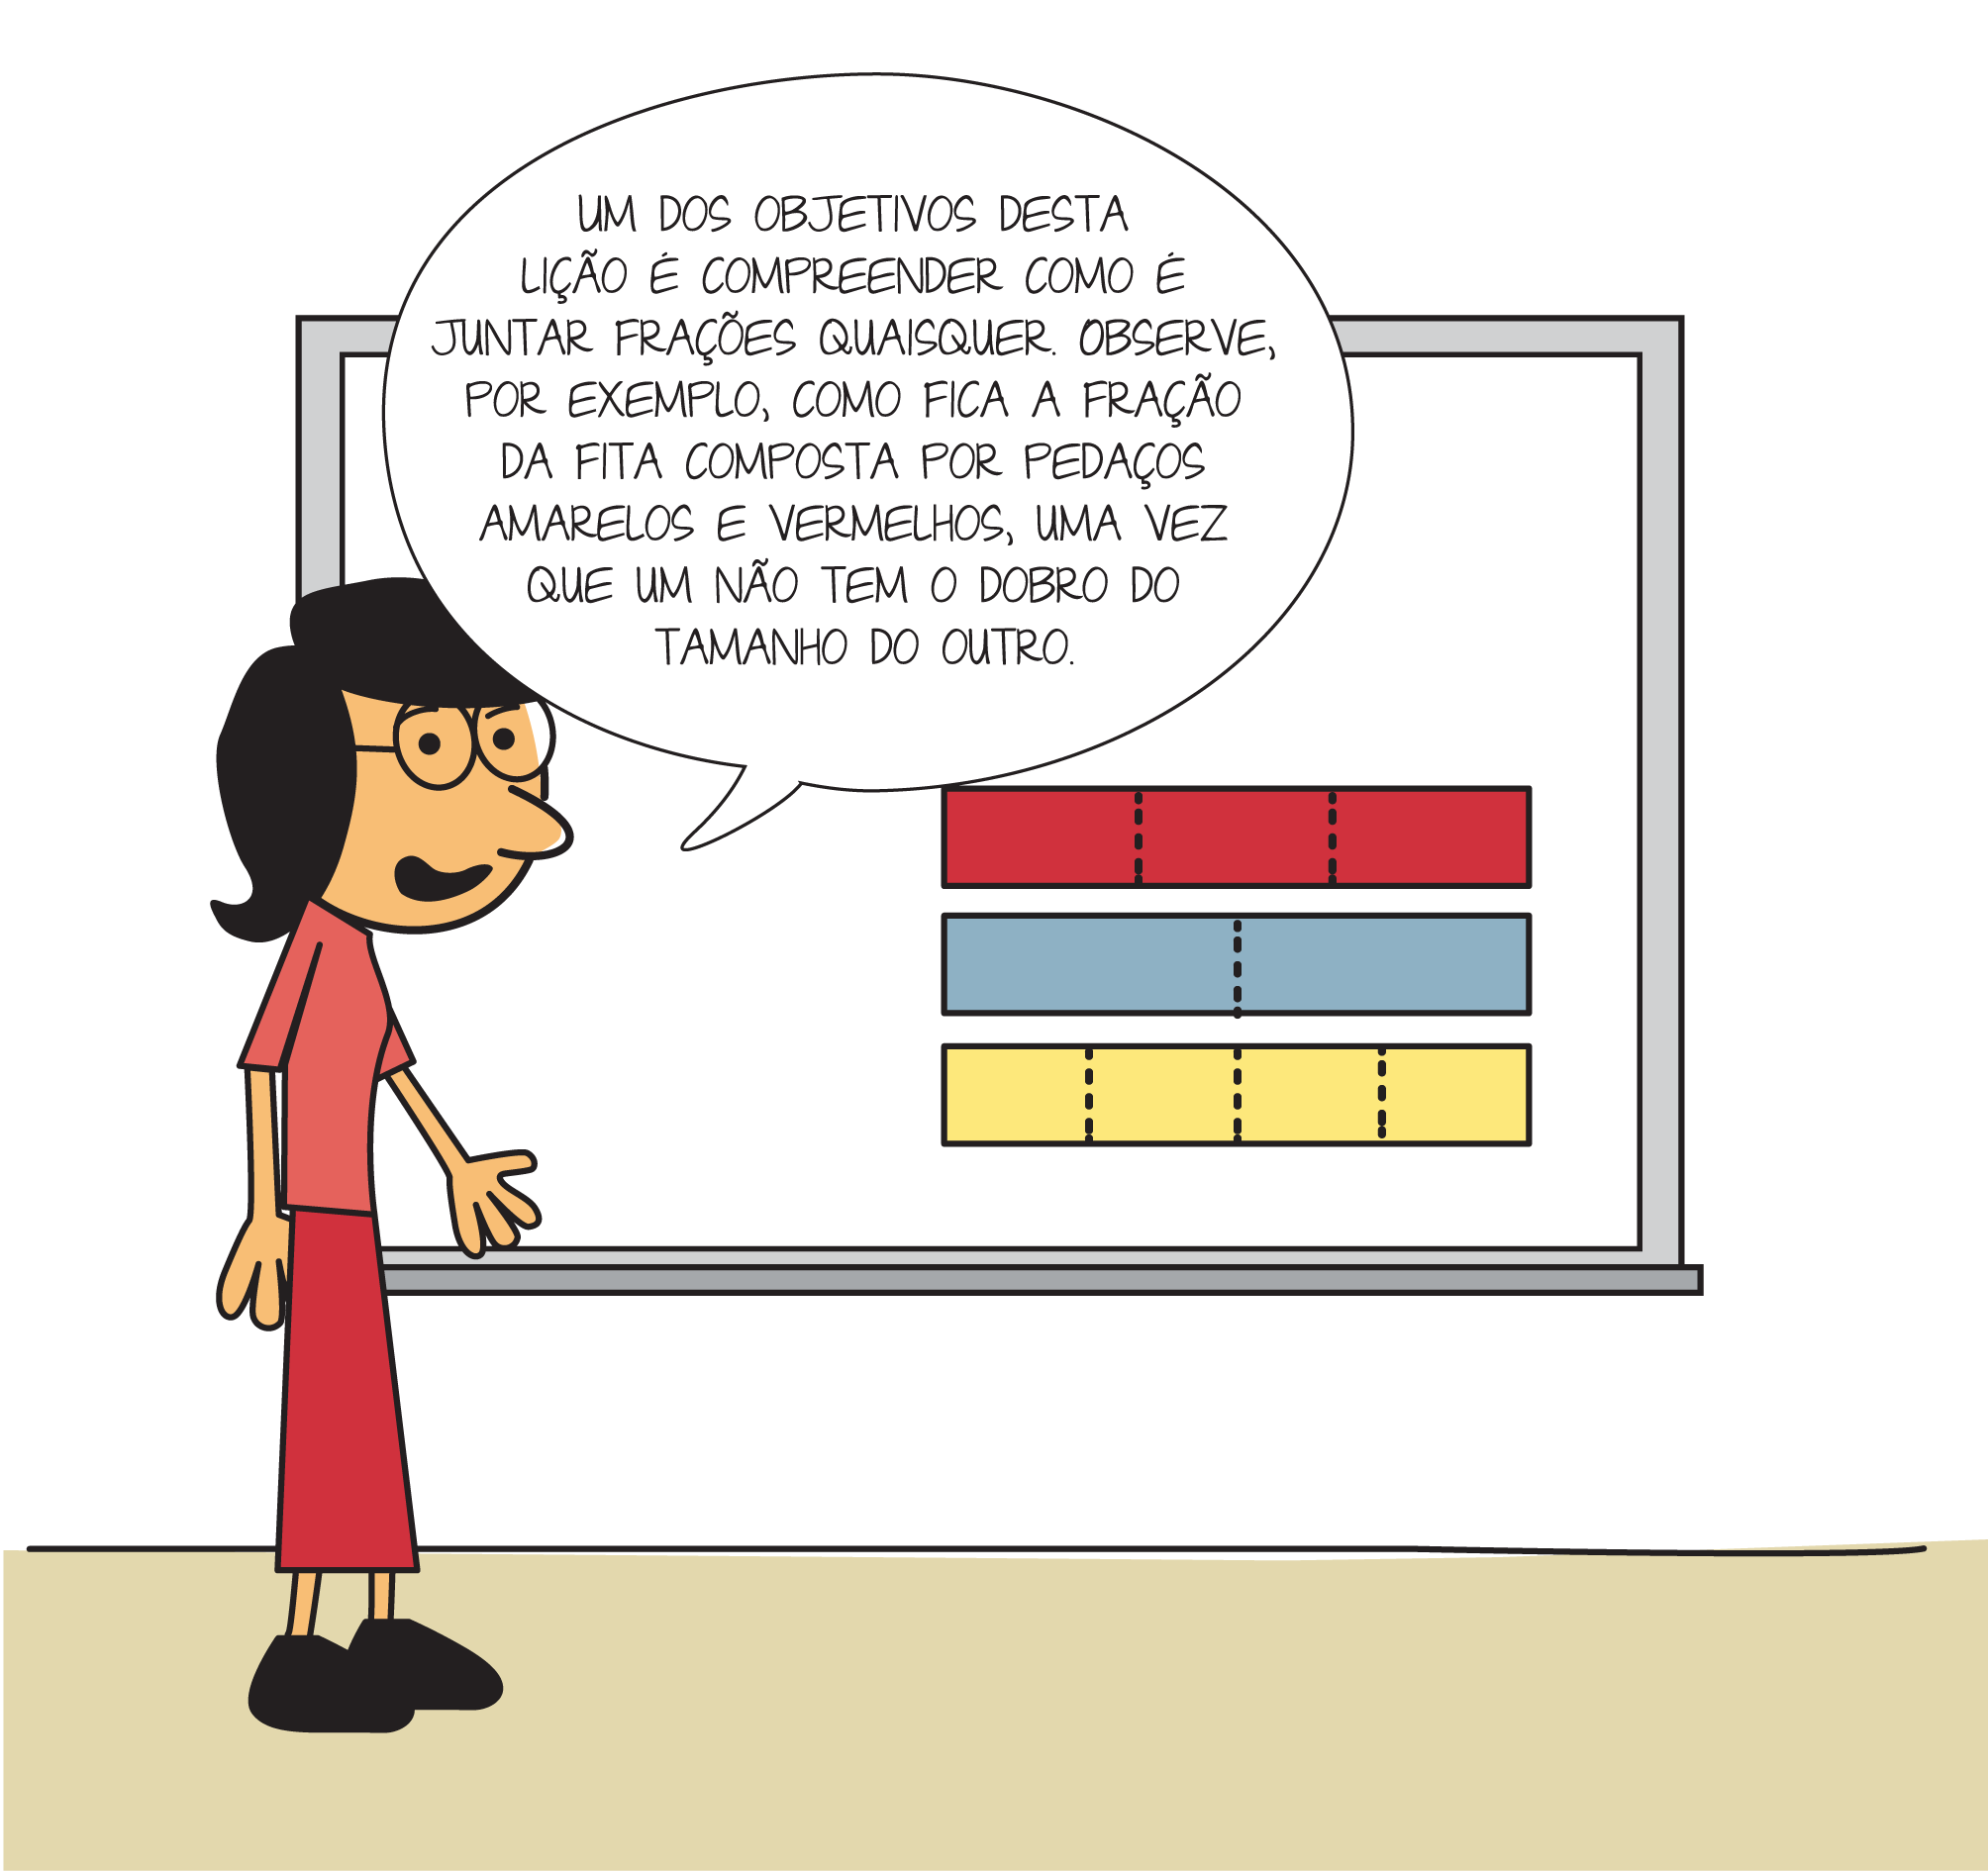
\includegraphics[width=330pt, keepaspectratio]{ativ2_fig01.png}
\end{center}

\ifdefined\prof
\begin{solucao}

\begin{enumerate}
    \item       Um pedaço vermelho recortado, corresponde a       $\frac{1}{3}$       da fita.       \mbox{} \newline        Um pedaço azul recortado, corresponde a       $\frac{1}{2}$       da fita.       \mbox{} \newline        Um pedaço amarelo recortado, corresponde a       $\frac{1}{4}$       da fita.
  \item       Um pedaço amarelo mais um pedaço azul corresponde a       $\frac{1}{4} +\frac{1}{2}$       da fita. Como       $\frac{1}{2} =\frac{2}{4}$, temos que a junção dos dois pedaços de fita será       $\frac{1}{4} +\frac{1}{2} = \frac{3}{4}$       da tamanho da fita original.
\end{enumerate}

\end{solucao}
\fi

\end{document}